%%%%%%%%%%%%%%%%%%%%%%%%%%%%%%%%%%%%%%%%%%%%%%%%%%%%%%%%%%%%%%%%%%%%%%%%%%%%%%%%
\chapter{Анализ подходов}
%%%%%%%%%%%%%%%%%%%%%%%%%%%%%%%%%%%%%%%%%%%%%%%%%%%%%%%%%%%%%%%%%%%%%%%%%%%%%%%%

\section{Подход 1}

\subsection{Инструмент 1}

Ссылка на статью \cite{russian}

Ссылка на сайт \cite{ANTLR}

\nomenclature{АСД}{Абстрактное синтаксическое дерево, AST}

\section{Подход 2}

Ссылка на книгу \cite{java-book}

Ссылка на рисунок \ref{fig:idea}

\begin{figure}[htbp]
	\centering
	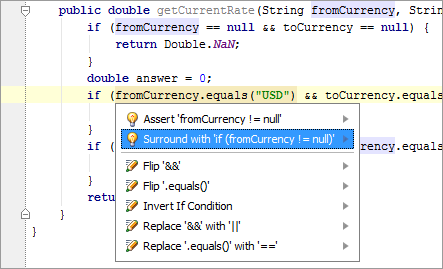
\includegraphics[width=0.8\textwidth]{fig/code_analysis_bugs.png}
	\caption{Предупреждение от статического анализатора в IntelliJ IDEA и всплывающее меню Quick Fix}%
	\label{fig:idea}
\end{figure}